\documentclass[../cheatSheetAlgoritmi.tex]{subfiles}
\begin{document}

\chapter{Backtracking}
\section{Introduzione}
In alcuni problemi è richiesto oppure è necessario analizzare l'intero spazio delle soluzioni ammissibili, in particolare possiamo usufruire della tecnica di backtracking ogni volta in cui ci è richiesto di:
\begin{itemize}
	\item elencare \textcolor{red}{tutte} le soluzioni \textcolor{red}{\emph{ammissibili}} (problemi di enumerazione)
	\item trovare  \textcolor{red}{una} soluzione \textcolor{red}{\emph{ammissibile}} in uno spazio di soluzioni molto grandi, dove una volta trovata è possibile uscire dalla procedura (problemi di ricerca)
	\item contare  \textcolor{red}{tutte} le soluzioni \textcolor{red}{\emph{ammissibili}} (problemi di conteggio), questo infatti viene effettuato per tutti i problemi in cui non si conosce o non è possibile avere una formula che stabilisce la dimensione dell'insieme delle soluzioni in maniera analitica.
	\item trovare \textcolor{red}{una} delle soluzioni \textcolor{red}{\emph{ammissibili}} migliori rispetto ad un certo criterio di valutazione (problemi di ottimizzazione)
\end{itemize}
Analizzare tutte le possibili soluzioni è ovviamente molto costoso in quanto lo spazio delle possibili soluzioni può avere dimensione superpolinomiale, anche se a volte è l'unica soluzione deterministica possibile. Fortunatamente, in alcuni casi, è possibile ridurre lo spazio delle soluzioni effettivamente analizzate, nonostante la complessità computazionale rimanga di fatto invariata. 

\section{Tecnica di backtracking}
Durante il corso abbiamo visto due possibili modalità per implementare la tecnica di backtracking: 
\begin{itemize}
	\item La \textbf{ricorsione}, un metodo sistematico per esplorare lo spazio di ricerca salvando le scelte fatte fino ad ora grazie ad una struttura dati passata come parametro alla procedura
	\item L'\textbf{iterazione}, un approccio greedy dove è possibile ritornare sui propri passi.
\end{itemize}
\textbf{Organizzazione generale} 
\begin{itemize}
	\item Una soluzione viene rappresentata come un vettore di scelte $S[1...n]$ (ovviamente in base al problema da risolvere è possibile utilizzare una struttura dati differente)
	\item Il contenuto degli elementi $S[i]$ è preso da un insieme di scelte $C$ dipendente dal problema
\end{itemize}

\section{Enumerazione}
Lo schema parziale per la risoluzione di problemi di enumerazione potrebbe essere il seguente: 
 \begin{lstlisting}[ caption= Schema generale risoluzione problema di enumerazione]
enumeration($\langle$dati del problema$\rangle$, ITEM[] S, int i, $\langle$dati parziali$\rangle$)
	% Verifica se S[i...i - 1] contiene una soluzione ammissibile
	if accept($\langle$dati del problema$\rangle$, S, i, $\langle$dati parziali$\rangle$) then
		% "Processa" la soluzione (stampa, conta, etc.)
		processSolution($\langle$dati problema$\rangle$, S, i, $\langle$dati parziali$\rangle$)
	else
		% Calcola l'insieme delle scelte in funzione di S[1... i - 1]
		SET C = choices($\langle$dati problema$\rangle$, S, i, $\langle$dati parziali$\rangle$)
		% Itera sull'insieme delle scelte
		foreach $c \in C$ do
			S[i] = c %Scelta fatta
			% Chiamata ricorsiva
			enumeration($\langle$dati problema$\rangle$, S, i + 1, $\langle$dati parziali$\rangle$)
\end{lstlisting}
Le caratteristiche di tale schema sono le seguenti: 
\begin{itemize}
	\item Il parametro $i$ rappresenta l'indice della prossima decisione da prendere
	\item La soluzione parziale $S[1...i - 1]$ contiene le decisioni prese finora
	\item \textcolor{red}{Caso base}:
	\begin{itemize}
		\item Se $S[1... i - 1]$ è una soluzione ammissibile, questa viene processata
		\item Assumendo che le soluzioni ammissibili non possano essere estese, la ricorsione termina
	\end{itemize}
	\item \textcolor{red}{Passo ricorsivo}
	\begin{itemize}
		\item Altrimenti, calcoliamo l'insieme $C$ delle scelte possibili
		\item Per ogni elemento $c \in C$:
		\begin{itemize}
			\item Scriviamo $c$ sulla scelta $S[i]$
			\item Chiamiamo ricorsivamente la funzione con indice $i+ 1$
		\end{itemize}
	\end{itemize}
\end{itemize}
L'esporazione dello spazio delle soluzioni, ammissibili e non, da origine a quello che viene chiamato \textcolor{red}{Albero delle decisioni}, che ha le seguenti caratteristiche:
\begin{itemize}
	\item \textcolor{red}{Albero di decisione} $\equiv$ Spazio di ricerca
	\item  \textcolor{red}{Radice} $\equiv$ Soluzione parziale vuota
	\item  \textcolor{red}{Nodi interni dell'albero di decisione} $\equiv$ Soluzioni parziali
	\item  \textcolor{red}{Foglie in un albero di decisione} $\equiv$ Soluzioni ammissibili
\end{itemize}
\begin{center}
	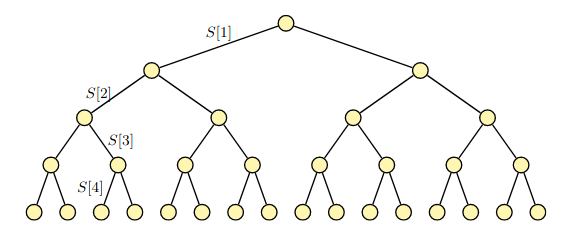
\includegraphics{../img/backtracking_albero_delle_decisioni}
\end{center}
Grazie ad alcuni accorgimenti è possibile evitare di attraversare i rami dell'albero delle decisioni che sicuramente porteranno a soluzioni non ammissibili, questa tecnica è detta \emph{potatura} o \emph{pruning}.

\section{Sottoinsiemi}
Un esempio di problema di enumerazione potrebbe essere quello di elencare tutti i possibili sottoinsiemi dell'insieme $\{ 1, ..., n\}$
 \begin{lstlisting}[ caption= Schema generale enumerazione subsets]
 subsets(int n)
	int[] S = new int[1...n]
 	subsetsRec(n, S, 1) 
 	
 subsetsRec(int n, int[] S, int i)
 	% S ammissibile dopo n scelte
 	if i > n then
 		processSolution(S, n)
 	else 
 		% Non presente, presente (prendere o non prendere)
 		SET C = {0, 1}
 		foreach $c \in C$ do
 			S[i] = c
 			subsetsRec(n, S, i + 1)
 
processSolution(int[] S, int n)
	print "{"
		for i = 1 to n do
			if S[i] then
				print i, " "
	print "}"
\end{lstlisting}
In questo problema, come viene di fatto richiesto è stato esplorato tutto lo spazio possibile delle soluzioni. La complessità risulta essere dunque $\Theta(n \cdot 2^n)$, dato che vengono generati $2^n$ sottoinsiemi, e per ogniuno di essi è necessario effettuare l'operazione di stampa di costo $\mathcal{O}(n)$. \\
La soluzione è memorizzata all'interno di un vettore $S[1 ... n]$ il quale salverà nella cella $i$-esima le scelte $0$ (elemento $i$-esimo non compreso) oppure $1$ (elemento i-esimo compreso). L'insieme di possibili scelte che possono essere effettuate nel passo ricorsivo non cambia a seconda della soluzione e sono rappresentate dal SET C che contiene, come era intuibile, i valori $\{0, 1\}$. \\
Una volta effettuata una scelta (tutte le scelte alla fine dovranno essere prese) la si salva nela cella dedicata all'elemento corrente della soluzione $S[i]$ e si prosegue con le chiamate ricorsive.
Si osserva che la ricorsione termina quando $i > n$, ovvero sono stati analizzati tutti gli elementi dell'insieme $\{1...n\}$, dove la soluzione verrà processata. \\
È possibile risolvere questo problema anche in maniera iterativa, la soluzione proposta è la seguente:
 \begin{lstlisting}[ caption= Schema generale enumerazione subsets iterativa]
 subsets(int n)
	for j = 0 to $2^n - 1$ do
		print "{ "
		for i = 0 to n - 1 do
			if (j && $2^i$) $\neq 0$ then % And bit a bit (bitwise and)
				print i, " "
		print "}"
\end{lstlisting}
La complessità rimane invariata: $\Theta(n \cdot 2^n)$. 

\section{Permutazioni}
Un altro esempio di problema di enumerazione è quello che prevede di stampare tutte le permutazioni di un insieme $A$.
 \begin{lstlisting}[ caption= Schema generale permutazioni]
 permutations(SET A)
	int n = size(A)
	int[] S = new int[1...n]
	permRec(A, S, 1)

permRec(SET A, ITEM[] S, int i)
	% Se A risulta vuoto, S e' ammissibile
	if A.isEmpty() then
		print S
	else
		% Copia A per il ciclo foreach
		SET C = copy(A)
		foreach $c \in C$ do
			S[i] = c
			A.remove(c)
			permRec(A, S, i + 1)
			A.insert(c)
\end{lstlisting}
In quanto parliamo di permutazioni non possiamo usare lo schema precedente, è necessario infatti conoscere quale scelta è stata precedentemente fatta. Questo viene fatto grazie ad un SET $A$ passato per parametro. \\
Ad ogni scelta viene copiato tale insieme per poter effettuare tutte le possibili scelte, ad ogni decisione è necessario notificare agli elementi successivi che tale elemento non è più disponibile, rimuovendo l'elemento scelto dal SET $A$, passando $A$ alla chiamata successiva (il prossimo passo non avrà tale scelta tra quelle possibili), ad una decisione nuova invece viene reso tale valore nuovamente disponibile reinserendolo nel set. \\
La complessità per il calcolo delle permutazioni può essere calcolato sviluppando l'albero delle decisioni, in particolare possiamo ricavare che:
\begin{itemize}
	\item Costo della stampa: $\Theta(n)$
	\item Il costo delle copie del vettore lungo un cammino radice-foglia:
	$\sum_{i = 1}^{n} O(i) = O(n^2)$
	\item Il numero di foglie è: $n!$
	\item La complessità è dunque $\mathcal{O}(n^2n!)$
\end{itemize}
È possibile ridurre il costo computazionale per il calcolo delle permutazioni se riusciamo ad evitare il costo di copia del set, un modo possibile potrebbe essere il seguente:
 \begin{lstlisting}[ caption= Schema generale permutazioni migliorata]
 permutations(ITEM[] S, int n)
	permRec(S, n)

permRec(ITEM[] S, int i)
	% Caso base un elemento
	if i $==$ 1 then
		print S
	else
		% Non copiamo l'intero set, bensi' facciamo degli scambi di elmenti
		for j = 1 to i do
			swap(S, i, j)
			permRec(S, i - 1)
			swap(S, i, j)
\end{lstlisting}
Il funzionamento è analogo al precedente solamente che effettua tutti i possibili scambi di elementi dell'insieme al posto di utilizzare un set per le scelte possibili. \\
In questo caso si ha:
\begin{itemize}
	\item $n!$ permutazioni
	\item $\Theta(n)$ per stamparle tutte
	\item $2n$ swap per ogni permutazione
	\item Il costo totale è dunque: $\Theta(n \cdot n!)$
\end{itemize}

\section{Enumerazione conclusione}
Lo schema conclusivo per tutti i problemi di enumerazione, da adattare al caso specifico, è il seguente:
 \begin{lstlisting}[ caption= Schema generale enumerazione completo]
enumeration($\langle$dati del problema$\rangle$, ITEM[] S, int i, $\langle$dati parziali$\rangle$)
	% Verifica se S[i...i - 1] contiene una soluzione ammissibile
	if accept($\langle$dati del problema$\rangle$, S, i, $\langle$dati parziali$\rangle$) then
		% "Processa" la soluzione (stampa, conta, etc.)
		processSolution($\langle$dati problema$\rangle$, S, i, $\langle$dati parziali$\rangle$)
	% Se la soluzione non e' ammissibile allora viene scartata
	else if reject($\langle$dati problema$\rangle$, S, i, $\langle$dati parziali$\rangle$) then
		return
	else
		% Calcola l'insieme delle scelte in funzione di S[1... i - 1]
		SET C = choices($\langle$dati problema$\rangle$, S, i, $\langle$dati parziali$\rangle$)
		% Itera sull'insieme delle scelte
		foreach $c \in C$ do
			S[i] = c %Scelta fatta
			% Chiamata ricorsiva
			enumeration($\langle$dati problema$\rangle$, S, i + 1, $\langle$dati parziali$\rangle$)
\end{lstlisting}

\section{Sottoinsiemi di k elementi}
Un ulteriore problema di enumerazione è quello di elencare tutti i possibili insiemi di $k$ elementi di un insieme $\{1, ..., n\}$. \\
Possiamo affrontarlo utilizzando lo schema introdotto poc'anzi.
 \begin{lstlisting}[ caption= Sottoinsiemi di k elementi inefficiente]
kSubsets(int n, int k)
	int[] S = new int[1 ... n]
	kssRec(n, k, S, 1)

kssRec(int n, int k, int[] S, int i)
	int size = count(S, n)
	if i > n and size $==$ k then
		processSolution(S, n)
	else if i > n and size $\neq$ k then
		return 
	else
		foreach $c \in \{0, 1\}$ do
			S[i] = c
			kssRec(n, k, S, i + 1)
			
int count(int[] S, int n)
	int count = 0
	for j = 1 to n do
		count = count + S[j]
	return count
\end{lstlisting}
La soluzione ammissibile è salvata all'interno del vettore $S$. \\
Ad ogni passo ricorsivo si decide se inserire o meno l'elemento i-esimo all'interno della soluzione scegliendo tra i valori $0$ (elemento non compreso) e $1$ (elemento compreso).  \\
Ogni volta che una scelta viene effettuata viene registrata all'interno del vettore $S$ e si passa all'analisi del prossimo valore. \\
Viene contato il numero di elementi compresi nella soluzione attraverso la funzione \emph{count}: se abbiamo terminato di analizzare l'intero insieme e la dimensione è pari a $k$ allora processiamo la soluzione, altrimenti se abbiamo terminato l'analisi e la cardinalità di $S$ è superiore a $k$ la scartiamo, se invece abbiamo ancora elementi da scansionare proseguiamo con le scelte. \\
Possiamo, invece che contare ogni volta il numero di elementi inseriti, utilizzare una variabile missing, la quale sarà inizializzata a $k$ ed identifica il numero di elementi che sono necessari per completare la soluzione corrente. \\ 
Come nella soluzione precedente, se terminata l'analisi dell'insieme $missing$ è pari a $0$ allora processiamo la soluzione (abbiamo inserito esattamente $k$ elementi) altrimenti la scartiamo, se mancano dei numeri da scandire allora effettueremo la scelta decrementando $missing$ di $1$, se abbiamo deciso che l'elemento $i$-esimo è compreso in $S$, oppure lasciandolo invariato, se si è deciso di non comprenderlo nella soluzione. 
 
\begin{flushleft}
Una maniera più intelligente per implementare la procedura \emph{kssRec} è la seguente:
\end{flushleft}
\begin{lstlisting}[ caption= K-subsets migliore]
kSubsets(int n, int k)
	int[] S = new int[1 ... n]
	return kssRec(n, k, S, 1)

kssRec(int n, int missing, int[] S, int i)
	if i > n and missing $==$ 0 then
		processSolution(S, n)
	else if i > n and missing $\neq$ 0 then
		return 
	else
		foreach $c \in \{0, 1\}$ do
			S[i] = c
			kssRec(n, missing - c, S, i + 1)
\end{lstlisting}
Possiamo ridurre la dimensione dell'albero delle decisioni (pruning) facendo un ulteriore accorgimento, ovvero facendo in  modo di scartare a priori soluzioni che non porteranno mai ad un risultato corretto. \\
Infatti non ha senso arrivare fino alla scansione dell'ultimo elemento prima di poter scartare la soluzione errata, è sufficiente controllare che il valore $missing$ sia maggiore o uguale di $0$. \\
Se $missing = 0$ abbiamo trovato una soluzione ammissibile, se $missing < 0$ oppure siamo arrivati al termine degli elementi con $missing > 0$, il che significa che non possiamo completare il SET con i $k$ elementi richiesti, scartiamo la soluzione. \\
Se $missing > 0$ e abbiamo altri elementi da analizzare allora possiamo continuare con le scelte:
 \begin{lstlisting}[ caption= K-subsets pruning parziale]
kSubsets(int n, int k)
	int[] S = new int[1 ... n]
	return kssRec(n, k, S, 1)

kssRec(int n, int missing, int[] S, int i)
	if missing $==$ 0 then
		processSolution(S, i - 1)
	else if i > n or missing < 0 then
		return 
	else
		foreach $c \in \{0, 1\}$ do
			S[i] = c
			kssRec(n, missing - c, S, i + 1)
\end{lstlisting}
È 	possibile ottenere un \emph{pruning} totale facendo un ulteriore accorgimento nel caso in cui il $missing > 0$. \\
Se abbiamo altri valori da analizzare e con gli elementi rimasti non siamo in grado, nemmeno scegliendoli tutti, di riempire $S$ con esattamente $k$ elementi allora è possibile scartare la soluzione corrente ($n - (i - 1) < missing$).  
 
 \begin{lstlisting}[ caption= K-subsets pruning totale]
kSubsets(int n, int k)
	int[] S = new int[1 ... n]
	return kssRec(n, k, S, 1)

kssRec(int n, int missing, int[] S, int i)
	if missing $==$ 0 then
		processSolution(S, i - 1)
	else if i > n or missing < 0 or n - (i - 1) < missing then
		return 
	else
		foreach $c \in \{0, 1\}$ do
			S[i] = c
			kssRec(n, missing - c, S, i + 1)
\end{lstlisting}
La stessa soluzione ma più compatta è rappresentata qui sotto:
 \begin{lstlisting}[ caption= K-subsets pruning totale compatta]
kSubsets(int n, int k)
	int[] S = new int[1 ... n]
	return kssRec(n, k, S, 1)

kssRec(int n, int missing, int[] S, int i)
	if missing $==$ 0 then
		processSolution(S, i - 1)
	else if i $\leq$ n and $0 < missing  \leq n - (i - 1) $ then
		foreach $c \in \{0, 1\}$ do
			S[i] = c
			kssRec(n, missing - c, S, i + 1)
\end{lstlisting}

\section{Enumerazione con interruzione alla prima soluzione}
Ci sono dei problemi che non richiedono esplicitamente di analizzare l'intero spazio delle soluzioni, ma solamente di avere una soluzione ammissibile al problema. In questi casi è possibile utilizzare backtrack ma con una condizione di arresto al primo risultato accettabile. Uno schema per implementare quanto detto è il seguente:
 \begin{lstlisting}[ caption= Schema generale risoluzione problema di enumerazione con interruzione]
boolean enumeration($\langle$dati del problema$\rangle$, ITEM[] S, int i, $\langle$dati parziali$\rangle$)
	if accept($\langle$dati del problema$\rangle$, S, i, $\langle$dati parziali$\rangle$) then
		processSolution($\langle$dati problema$\rangle$, S, i, $\langle$dati parziali$\rangle$)
		return true	% Soluzione trovata, restituisco true
	else if reject($\langle$dati problema$\rangle$, S, i, $\langle$dati parziali$\rangle$) then	
		return false	% Soluzione non trovata, restituisco false
	else
		SET C = choices($\langle$dati problema$\rangle$, S, i, $\langle$dati parziali$\rangle$)
		foreach $c \in C$ do
			S[i] = c %Scelta fatta
			% Chiamata ricorsiva
			if enumeration($\langle$dati problema$\rangle$, S, i + 1, $\langle$dati parziali$\rangle$) then
				return true
		return false
\end{lstlisting}

\section{Subset sum backtracking}
Il problema è il seguente: Dati un vettore $A$ contenente $n$ interi positivi ed un intero positivo $k$, esiste un sotto insieme $S \subseteq \{1. . . n\}$ tale che $\sum_{i \in S} a[i] = k$? \\
Un modo per risolvere il problema, senza usare programmazione dinamica, è quello di usare una tecnica di backtracking che risolve il problema con complessità $\mathcal{O}(2^n)$. Tuttavia non siamo interessati a tutte le possibili soluzioni, ma solamente ad una, è quindi sufficiente utilizzare lo schema di risoluzione visto precedentemente in modo da fermare l'esecuzione quando si trova la prima soluzione valida:
 \begin{lstlisting}[ caption= Subset sum]
subsetSum(int[] A, int n, int k)
	int[] S = new int[1 ... n]
	ssRec(A, n, k, S, 1)

boolean ssRec(int[] A, int n, int missing, int[] S, int i)
	if missing $==$ 0 then
		processSolution(S, i - 1)
		return true
	else if i > n or missing < 0 then
		return false
	else 
		foreach $c \in \{0, 1\}$ do
			S[i] = c
			if ssRec(A, n, missing - A[i] $\cdot$ c, S, i + 1) then
				return true
		return false
\end{lstlisting}
Anche in questo caso come nel problema dei \emph{Subsets di k elementi}, usiamo una variabile $missing$ che indica il valore mancante da sommare per ottenere il valore $k$ richiesto. \\
Se $missing = 0$ significa che abbiamo trovato una soluzione valida, dove la somma degli elementi da come risultato $k$ e quindi terminiamo la procedura, se abbiamo terminato gli elementi disponibili da scegliere e $missing > 0$ oppure nel caso in cui $missing < 0$ la soluzione trovata non è ammissibile, mentre se abbiamo ancora valori da scandire e $missing > 0$ allora procediamo con le scelte.

\section{Il problema delle otto regine}
Anche in questo caso siamo interessati alla prima soluzione valida e quindi utilizziamo un approccio basato su backtrack come per il precedente. 
Nello specifico il problema è il seguente: \\
Dobbiamo posizionare $n$ regine in una scacchiera $n \times n$, in modo tale che nessuna regina ne "minacci" un'altra, ovvero che non ci siano regine che stiano sulla stessa riga, colonna e diagonale di un'altra.\\
I passi che ci hanno portato alla soluzione finale sono stati i seguenti:
\begin{itemize}
	\item Il primo approccio (inefficiente) è stato quello di cercare di posizionare $n$ regine su $n^2$ caselle, controllando la soluzione quando abbiamo analizzato l'ultima cella. Lo spazio della soluzione è comunque troppo grande, il costo è di $\mathcal{O}((n^2)^n)$.
	\item Il secondo miglioramento lo si ha avuto imponendo come vincolo il fatto di non posizionare le regine in caselle precedenti a quelle già scelte: lo spazio delle soluzioni si è ridotto di molto con un costo pari a  $\mathcal{O}\cfrac{(n^2)^n}{n!}$ (comunque ancora troppo elevato).
	\item Posizionare una regina su ogni riga ha consentito un altro avanzamento in quanto, anche a livello intuitivo, le $n$ regine dovranno necessariamente trovarsi su righe differenti della scacchiera: la complessità in questo caso è $\mathcal{O}(n^n)$.
	\item Il miglioramento finale è stato quello di vincolare la scelta di colonne differenti, in quanto le $n$ regine devono trovarsi necessariamente in colonne distinte. La complessità è stata dunque ridotta a: $\mathcal{O}(n!)$
\end{itemize}
Per evitare di essere troppo prolissi ci concentreremo solamente sulla soluzione discussa nell'ultimo punto (di fatto la più efficiente). \\
Le caratteristiche di questa soluzione sono le seguenti: 
\begin{itemize}
	\item La soluzione del problema è memorizzata in $S[1 ... n]$, dove sono salvate le colonne, mentre l'indice rappresenta la riga dove le regine risiedono, ovvero in $S$ sarà presente una permutazione dei valori $\{1 ... n\}$, rispettando già nella scelta il vincolo che sulla stessa riga e sulla stessa colonna di una qualsiasi regina non può risiedervi un'altra.
	\item La soluzione sarà controllata nel momento in cui si arriva all'ultimo elemento considerato, dunque se $i = n$
	\item La funzione \emph{choices(S, n, i)} si occuperà di restituire le scelte possibili: nel nostro caso dovrà ritornare $\{1 ... n\}$. È necessario che questa funzione controlli ogni scelta possibile generata a partire dalla soluzione parziale, ritornando solamente le colonne $c$ che non generano conflitti, ovvero che non siano già state occupate e, se assegnata alla regina $i-esima$, la posizione (i, c) non si trovi sulla diagonale di un'altra regina.
	\item È possibile effettuare del pruning eliminando le diagonali in quanto non possono esserci delle regine che stanno sulla stessa diagonale.
\end{itemize}
L'algoritmo proposto dal docente è il seguente: \\
Esso non fa uso della funzione \emph{choices(S, n, i)} discussa in precedenza, tuttavia per ogni scelta possibile effettua del puning: se la scelta della colonna $j$ per la regina $i$ non porta ad una soluzione parzialmente corretta, questa viene scartata. \\
In particolare in questo caso per ogni possibile colonna si controlla se essa è già stata presa da una qualsiasi delle regine precedenti e se la scelta di tale valore da parte della i-esima regina non generi un conflitto (dovuto alla presenza di un'altra regina sulla diagonale). \\
Se non ci fossero scelte valide allora si ritorna indietro, analizzando una scelta diversa da quella effettuata in precedenza.
 \begin{lstlisting}[ caption= Problema delle regine]
queen(int n, int[] S, int i)
	if i > n then
		print S % Il controllo della soluzione avviene quando i = n
	else 
		for j = 1 to n do % Proviamo a piazzare la regina nella colonna j
			boolean legal = true
			for k = 1 to i - 1 do % Verifichiamo le regine precedenti (pruning)
				% Se le regine precedenti sono sulla stessa colonna o sulle diagonali della regina i-esima non proseguo, segnando la mossa come invalida
				if $S[k] == j$ or $S[k] == j + i - k$ or $S[k] == j -  i + k$ then
					legal = false 
			if legal then
				S[i] = j	% La scelta e' legale
				queens(n, S, i + 1) % Analizzo la prossima riga
\end{lstlisting}
Grazie al pruning nella scelta, è possibile affermare che se riusciamo a posizionare l'ennesima regina allora la soluzione trovata è ammissibile.

\bigskip
\textbf{Minimum-conflicts heuristic} \\
Il problema delle $n$ regine è molto costoso, anche se abbiamo lavorato parecchio per ridurne il costo computazionale. Molto spesso infatti è impensabile lanciare un algoritmo di tale pesantezza su input molto elevati, è possibile quindi adottare alcune euristiche che non garantiscono di trovare un risultato corretto (è possibile risolvere questo problema lanciando sull'output ritornato, un algoritmo che verifichi se sia o meno una soluzione accettabile, se non lo fosse si riesegue l'algoritmo e si ripete la procedura) ma eseguono in tempi molto minori rispetto ad una soluzione deterministica basata su backtracking. \\
La \emph{Minimum-conflicts heuristic} per il problema delle $n$ è così definita: \\
Si parte da una soluzione iniziale "ragionevolmente buona", e si muove il pezzo con il più grande numero di conflitti nella casella della stessa colonna che genera il numero minimo di conflitti. Si ripete fino a quando non ci sono più pezzi da muovere. \\
Questo algoritmo può essere eseguito in tempo lineare, ma come accennato poc'anzi, non garantisce che il risultato sia corretto.

\section{Sudoku}
Il problema del Sudoku non ha bisogno di presentazioni. \\
Come è intuibile (è nella sezione di backtracking) esiste una soluzione basata su backtrack per completare il gioco. \\
La soluzione proposta è la seguente: 
 \begin{lstlisting}[ caption= Sudoku]
boolean sudoku(int[][] S, int i)
	if i $==$ 81 then
		processSolution(S, n)
		return true
	int x = i mod 9
	int y = $\lfloor i/9 \rfloor$
	SET C = moves(S, x, y)
	int old = S[x][y]
	foreach $c \in C$ do
		S[x][y] = c
		if sudoku(S, i + 1) then
			return true
	S[x][y] = old
	return false
	
SET moves(int[][] S, int x, int y)
	SET C = new Set()
	if S[x][y] $\neq$ 0 then
		% Numero pre-inserito
		C.insert(S[x][y])
	else
		% Verifica conflitti
		for c = 1 to 9 do
			if check(S, x, y, c) then
				C.insert(c)
	return C
	
	
boolean check(int[][] S, int x, int y, int c)
	for j = 0 to 8 do
		if S[x][j] $==$ c then
			% Controllo sulla colonna
			return false
		if S[j][y] $==$ c then
			% Controllo sulla riga
			return false
	int $b_x$ = $\lfloor x/3 \rfloor$
	int $b_y$ = $\lfloor y/3 \rfloor$
	for $i_x = 0$ to 2 do
		for $i_y = 0$ to 2 do
			% Controllo sulla sottotabella
			if S[$b_x \cdot 3 + i_x$][$b_y \cdot 3 + i_y$] = c then
				return false
	return true 
\end{lstlisting}
Questo algoritmo termina quando si sono posizionati tutti i valori $i == 81$ (il Sudoku è una tabella formata da 9 tabelle $3 \times 3$). 
Per ogni decisione viene lanciata la procedura \emph{moves} che ritorna le sole mosse che non generano conflitti, cioè quelle per cui tale valore non sia già presente su una riga, su una colonna della griglia oppure all'interno della stessa tabella. \\ Se non sono più disponibili mosse che non generino conflitti si setta la vecchia mossa e si torna alla scelta precedente scegliendo un nuovo valore.

\section{Knight tour}
Si consideri ancora una scacchiera $n \times n$; lo scopo è trovare un "giro di cavallo", ovvero un percorso di mosse valide del cavallo in modo che ogni casella venga visitata al più una volta.
\begin{center}
	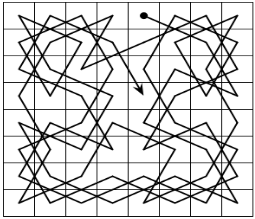
\includegraphics{../img/backtracking_knight_tour}
\end{center}
La soluzione, come di fatto è intuibile, è quella di utilizzare backtrack con un meccanismo che consente di determinare se una cella è stata o meno visitata come segue: \\
Nella matrice $n \times n$ vi saranno:
\begin{itemize}
	\item 0, se la cella non è mai stata visitata
	\item $i$, se la cella è stata visitata al passo i-esimo
\end{itemize}
 \begin{lstlisting}[ caption= Knight Tour]
boolean knightTour(int[][] S, int i, int x, int y)
	% Se i = 64, ho fatto 63 mosse e ho completato un tour (aperto)
	if i $==$ 64 then
		processSolution(S)
		return true
	SET C = moves(S, x, y)
	int[] $m_x$ = {-1, +1, +2, +2, +1, -1, -2, -2}
	int[] $m_y$ = {-2, -2, -1, +1, +2, +2, +1, -1}
	foreach $c \in C$ do
		S[x][y] = i
		if knightTour(S, i + 1, x + $m_x$[c], y + $m_y$[c]) then
			return true
		S[x][y] = 0
	return false
	
SET moves(int[][] S, int x, int y)
	SET C = new Set()
	int[] $m_x$ = {-1, +1, +2, +2, +1, -1, -2, -2}
	int[] $m_y$ = {-2, -2, -1, +1, +2, +2, +1, -1}
	for i = 1 to 8 do
		$n_x$ = x + $m_x$[i]
		$n_y$ = y + $m_y$[i]
		if $1 \leq n_x \leq 8$ and $1 \leq n_y \leq 8$ and $S[n_x][n_y] == 0$ then
			C.insert(i)
	return C
\end{lstlisting}
Le mosse sono generate a partire dal movimento del cavallo negli scacchi. \\
La procedura \emph{moves} controlla se la mossa vada a finire in una cella della matrice non visitata, se così non fosse non viene inserita all'interno del set. \\
Ad ogni passo si calcola il set di mosse che possono essere scelte, e per tutte queste si prova a completare il giro di cavallo: se si trova una soluzione la si processa in caso contrario si torna indietro settando la cella non visitata e riprovando con una nuova mossa tra quelle disponibili. \\
Se non rimane alcuna scelta valida si ritorna sui propri passi effettuando una scelta differente da quella effettuata in precedenza.

\bigskip
\textbf{Considerazioni sul problema}
\begin{itemize}
	\item Ad ogni passo ho al massimo $8$ caselle possibili, quindi ne visito al più $8^{63} \approx 7.8455$
	\item Grazie al pruning ne visito molto meno, ma resta comunque un problema non affrontabile per valori grandi di $n$
	\item È un esempio del più generale "problema del cammino hamiltoniano", per il quale non esistono soluzioni polinomiali
	\item Per questo particolare problema, tuttavia, esistono degli algoritmi di costo lineare nel numero di caselle, basati su divide-impera
\end{itemize}

\section{Inviluppo convesso}
\textbf{Definizioni:}
\begin{itemize}
	\item \textbf{Poligono convesso}: un poligono nel piano è \textcolor{red}{convesso} se ogni segmento di retta che congiunge due punti del poligono sta interamente nel poligono stesso (bordo incluso).
	\item \textbf{Inviluppo convesso}: dati $n$ punti $p_1, . . . , p_n$ nel piano, con $n \geq 3$, l'\textcolor{red}{inviluppo convesso} (\textcolor{red}{convex hull}) è, fra tutti i poligoni convessi che li contengono tutti, quello di superficie minima.
\end{itemize}
Ci chiediamo ora come è possibile determinare, dati $n$ punti ($n \geq 3$), quali tra questi costituiscano l'inviluppo convesso, ovvero quali debbano essere selezionati per costruire i bordi del poligono convesso di superficie minima contenente tutti gli $n$ punti.

\bigskip
\textbf{Soluzione} \\
Un primo approccio per risolvere il problema è quello di considerare retta che passa per una coppia di punti $p_i, p_j$, che divide il piano in due semipiani chiusi ($\mathcal{O}(n^2)$ coppie); infatti se tutti i punti rimanenti $(n - 2)$ stanno "dalla stessa parte", allora lo spigolo $S_{ij}$ fa parte dell'inviluppo convesso. Il costo di questa procedura sarà di $\mathcal{O}(n^3)$. Semplicemente lanciando per tutte le coppie di possibili di punti la procedura per determinare se tutti i punti rimanenti appartengono allo stesso semipiano, se si, allora tale coppia di vertici appartiene all'inviluppo convesso.
\begin{center}
	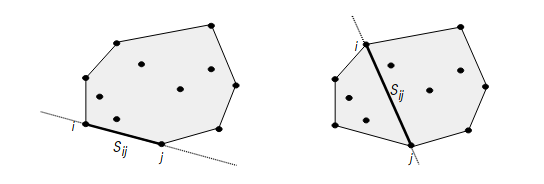
\includegraphics{../img/backtracking_inviluppo_convesso}
\end{center}
È necessario ora definire che significa stare dalla \emph{"stessa parte"}, ovvero tradurre in codice che vuol dire che i punti $p$ e $q$ stanno nello stesso semipiano definito dalla retta passante per i punti $p_1$ e $p_2$. \\
Possiamo fare questo utilizzando il seguente algoritmo:
 \begin{lstlisting}[ caption= Same Side (Inviluppo Convesso)]
boolean sameSide(POINT $p_1$, POINT $p_2$, POINT $p$, POINT $q$)
	float $d_x$ = $p_2$.x - $p_1$.x
	float $d_y$ = $p_2$.y - $p_1$.y
	float $d_{x1}$ = $p$.x - $p_1$.x
	float $d_{y1}$ = $p$.y - $p_1$.y
	float $d_{x2}$ = $q$.x - $p_2$.x
	float $d_{y2}$ = $q$.y - $p_2$.y
	return $((d_x \cdot d_{y1} - d_y \cdot d_{x1}) \cdot (d_x \cdot d_{y_2} - d_y \cdot d_{x_2}) \geq 0)$
\end{lstlisting}
Un algoritmo, più efficiente del primo approccio proposto, per trovare l'invippo convesso è quello di \emph{Jarvis} detto algoritmo di \emph{Gift Packing} la cui complessità è $\mathcal{O}(n \cdot h)$.

\section{Algoritmo di Jarvis}
Descriviamo il comportamento di questo algoritmo nelle tre macro aree che lo compongono:
\begin{itemize}
\item Inserimento dei primi punti nell'inviluppo convesso, i punti \{0, 1\}
	\begin{itemize}
		\item Si assegna a $p_0$ il punto più a sinistra, che appartiene sempre, all'inviluppo convesso ($\mathcal{O}(n)$ per la ricerca di tale punto)
		\item Si calcola l'angolo della retta passante per $p_0$ e ogni altro punto $p_{j}$ rispetto alla rettaverticale ($\mathcal{O}(n)$ in quanto è necessario calcolare l'angolo con tutti gli n - 1 punti)
		\item Si seleziona come punto $p_1$ il punto con angolo minore (costo $\mathcal{O}(n)$)
	\end{itemize}
\item Inserimento del punto $i$ generico
	\begin{itemize}
		\item Si considera la retta $r$ passante per i punti $p_{i - 1}$, $p_{i - 2}$
		\item Si calcola l'angolo passante per $p_{i - 1}$ e ogni altro punto non considerato e la retta $r$
		\item Si seleziona come punto $p_i$ il punto con angolo minore (esso apparterrà all'inviluppo convesso)
		\item Costo determinare ogni spigolo dell'inviluppo: $\mathcal{O}(n)$
	\end{itemize}
\item Terminazione dell'algoritmo
	\begin{itemize}
		\item La procedura termina, quando il punto con angolo minore rispetto al punto $p_{i-1}$ e la retta $r$ è il punto $p_0$ di partenza.
		\item L'algoritmo ha dunque costo $O(nh)$, dove $h$ è il numero di spigoli (numero di punti che fanno parte dell'inviluppo convesso)
	\end{itemize}
\end{itemize} 
Schema riassuntivo del funzionamento dell'algoritmo di Jarvis:
\begin{center}
	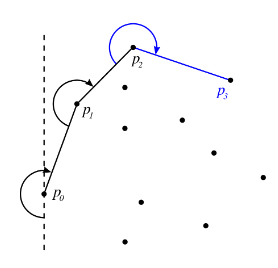
\includegraphics{../img/backtracking_inviluppo_convesso_jarvis}
\end{center}

\section{Algoritmo di Graham}
Un altro algoritmo per il calcolo dell'inviluppo convesso è l'algoritmo di Graham, il quale fa utilizzo di backtracking iterativo.
Il primo passo consiste nell'ordinare i punti seguendo le seguenti direttive:
\begin{itemize}
	\item Il punto con ordinata minima fa parte dell'inviluppo convesso (deve essere compreso dal poligono convesso)
	\item Si ordinano i punti in base all'angolo formato dalla retta passante per il punto con ordinata minima e la retta orizzontale
\end{itemize}
L'ordinamento per i vertici definito da Graham è rappresentato come segue:
\begin{center}
	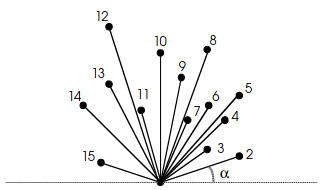
\includegraphics{../img/backtracking_inviluppo_convesso_graham_1}
\end{center}
Possiamo dunque inziare la stesura dell'algoritmo di Graham aggiungendo questa prima parte, con alcune considerazioni sui prossimi punti da prendere. 
 \begin{lstlisting}[ caption= Graham algorithm prima bozza]
STACK graham(POINT[] p, int n)
	int min = 1
	for i = 2 to n do
		if p[i].y < p[min].y then 
			min = i
	p[1] $\leftrightarrow$ p[min]
	{ riordina $p[2 ,..., n]$ in base all'angolo formato rispetto all'asse orizzontale quando sono connessi con $p[1]$}
	{ elimina eventuali punti allineati tranne i piu' lontani da $p_1$,aggiornando $n$}
\end{lstlisting}
Infatti, una volta inserito il primo vertice all'interno dell'inviluppo convesso, si procede come segue: ogni volta che viene selezionato un vertice, si controlla se, considerata la retta passante per gli ultimi due vertici inseriti, il punto $p_i$ considerato non è nello stesso piano del punto $p_1$ di riferimento (il primo inserito, quello che dovrà sempre fare parte dell'inviluppo) allora il punto $p_j$ non può appartenere all'inviluppo (altrimenti avrebbe determinato $p_1$ e $p_i$ dallo stesso piano sezionato dalla retta passante per $p_{j-1}$ e $p_j$) e quindi lo rimuoviamo dall'inviluppo corrente. Continuiamo questo controllo fino a quando $p_i$ e $p_1$ fanno parte dello stesso piano inserendo $p_i$ nell'inviluppo. \\
In altre parole:
\begin{itemize}
	\item Inseriamo $p_1$, $p_2$ nell'inviluppo corrente
	\item Per tutti i punti $p_i = 3, . . . , n$:
	\begin{itemize}
		\item Siano $p_{j - 1}$ e $p_j$ il penultimo e ultimo vertice dell'inviluppo corrente
		\item Se \emph{sameSide($p_{j - 1}$, $p_j$, $p_1$, $p_i$)} = \textbf{false}, ovvero $p_1$ e $p_i$ non si trovano dalla stessa parte rispetto alla retta passante per $p_{j - 1}$ e $p_j$, allora elimina $p_j$ dall'inviluppo corrente
		\item Termina tale "scansione" se $p_j$ non deve essere eliminato
		\item Aggiungi $p_j$, all'inviluppo "corrente"
	\end{itemize}
\end{itemize}
 \begin{lstlisting}[ caption= Graham algorithm]
STACK graham(POINT[] p, int n)
	int min = 1
	for i = 2 to n do
		if p[i].y < p[min].y then 
			min = i
	p[1] $\leftrightarrow$ p[min]
	STACK S = new Set()
	S.push($p_1$)
	S.push($p_2$)
	for i = 3 to n do
		while not sameSide(S.top(), S.top2(), $p_1$, $p_i$) do
			S.pop()
		S.push($p_i$)
	return S
\end{lstlisting}
\begin{center}
	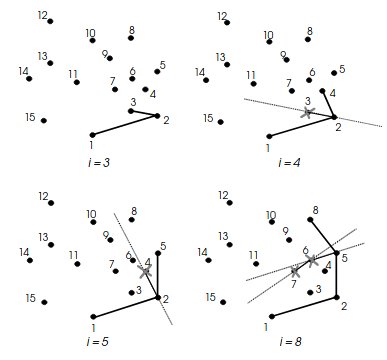
\includegraphics{../img/backtracking_inviluppo_convesso_graham_2}
\end{center}
La complessità è $\mathcal{O}(n \log n)$ dato da:
\begin{itemize}
	\item Il calcolo degli angoli richiede $\mathcal{O}(n)$
	\item L'ordinamento richiede $\mathcal{O}(n \log n)$
	\item La rimozione di punti con angolo uguale richiede $\mathcal{O}(n)$
	\item Ogni punto viene aggiunto/rimosso al massimo una volta (il costo è dunque $\mathcal{O}(n)$)
\end{itemize}
 
\end{document}